\subsection{Log-Sum-Exp}

\begin{figure*}[t]
    \centering
    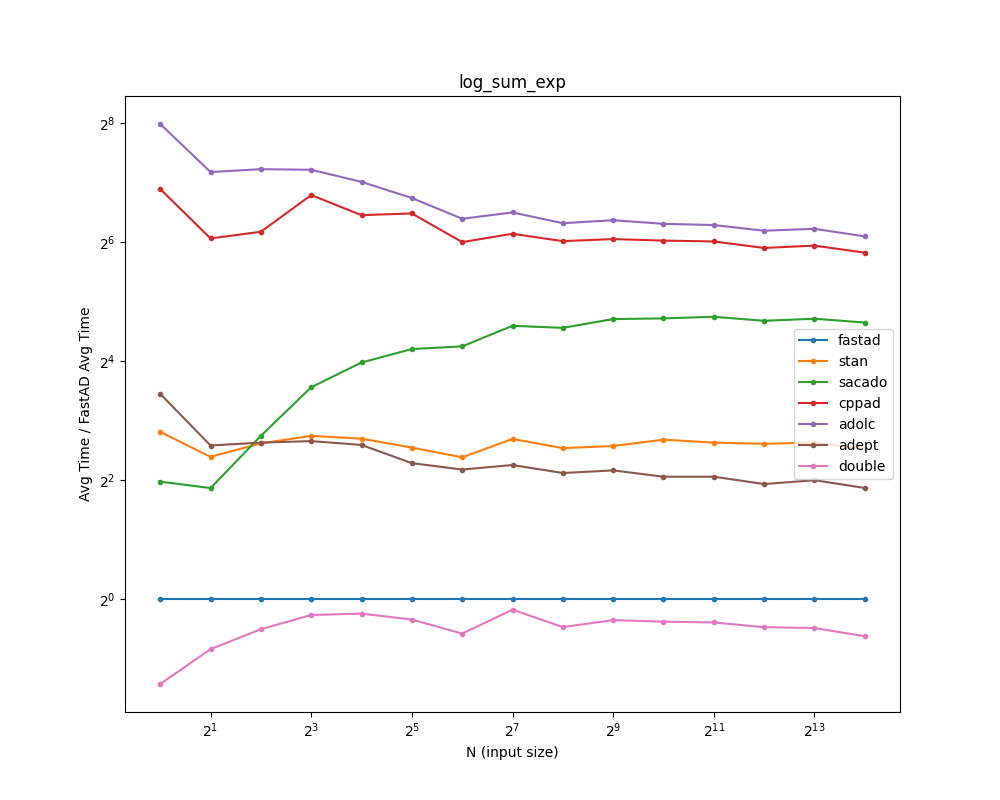
\includegraphics[width=0.8\textwidth]{figs/log_sum_exp_fig.png}
    \caption{%
        Log-sum-exp benchmark of other libraries against FastAD 
        plotted relative to FastAD average time.
    }\label{fig:log_sum_exp}
\end{figure*}

The log-sum-exp function is defined as $f:\R^n \to \R$ 
where~$f(x) = \log(\sum\limits_{i=1}^n e^{x_i})$,
Fig.~\ref{fig:log_sum_exp} shows the benchmark results.

FastAD outperforms all libraries for all values of $N$.
The next three fastest libraries are Adept, Stan, and CppAD, respectively.
The trend stabilizes starting from $N=2^6=64$ where 
Adept is about $ 2.5$ times slower than FastAD, 
and Stan about $ 7.7$ times.
Note that FastAD is only marginally slower than the baseline,
especially for small to moderate values of $N$,
despite calls to expensive functions like \code{log} and \code{exp}.
In fact, at the largest value of $N = 2^{14}$, 
FastAD is $ 1.5$ times slower than the baseline, 
meaning there is about $ 50\%$
overhead from one forward-evaluation to also compute the gradient.
This is because FastAD is optimized such that in this case
the forward-evaluated result for \code{exp} expression is reused
during the backward-evaluation.
